
\section{Algebraic Structures}

%\subsection{Software Design}

The algebraic structure concepts introduced within this section are 
motivated by their well known counterparts in traditional algebra, 
but we also had to pay tribute to existing types and their restrictions. 
To keep the interface minimal,
it was not desirable to cover all known algebraic structures, 
e.g., we did not introduce concepts for such basic structures as {\em groups} or
exceptional structures as {\em skew fields}. 

\begin{figure}[htbp]
\begin{ccTexOnly}
\begin{center}
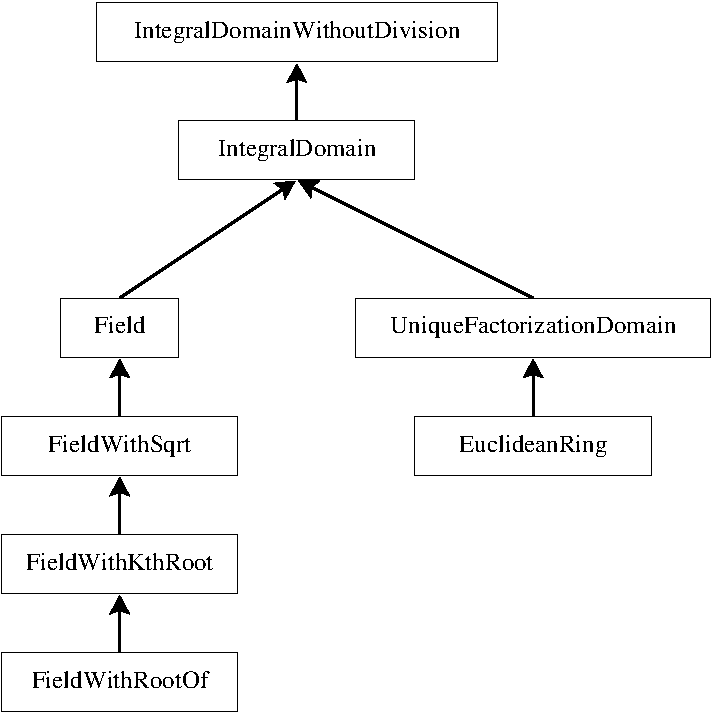
\includegraphics[width=3in]{Algebraic_foundations/fig/AlgebraicConceptHierarchy}
 %.ps(PS) .png(PDF)
\end{center}
\end{ccTexOnly}


\begin{ccHtmlOnly}
<CENTER>
<IMG BORDER=0 SRC="fig/AlgebraicConceptHierarchy.gif" 
 ALIGN=middle ALT="Concept Hierarchy of Algebraic Structures">
</CENTER>
\end{ccHtmlOnly}

\caption{Concept Hierarchy of Algebraic Structures
\label{fig::ConceptHierarchyOfAlgebraicStructures}}
\end{figure}

Figure~\ref{fig::ConceptHierarchyOfAlgebraicStructures} shows the refinement 
relationship of the algebraic structure concepts. 
\ccc{IntegralDomain}, \ccc{UniqueFactorizationDomain}, \ccc{EuclideanRing}  and 
\ccc{Field} correspond to the algebraic structures with the
same name. \ccc{FieldWithSqrt}, \ccc{FieldWithKthRoot} and 
\ccc{FieldWithRootOf} are fields that in addition are closed under 
the operations 'sqrt', 'k-th root' and 'real root of a polynomial', 
respectively. The concept \ccc{IntegralDomainWithoutDivision} also
corresponds to integral domains in the algebraic sense, the
distinction results from the fact that some implementations of
integral domains lack the (algebraically always well defined) integral 
division.
Note that \ccc{Field} refines \ccc{IntegralDomain}. This is because 
most ring-theoretic notions like greatest common divisors become trivial for 
\ccc{Field}s. Hence we see \ccc{Field} as a refinement of 
\ccc{IntegralDomain} and not as a 
refinement of one of the more advanced types of ring. 
If an algorithm wants to rely on gcd or remainder computation, it is trying 
to do things it should not do with a \ccc{Field} in the first place. 


The main properties of an algebraic structure are collected in the class   
\ccc{Algebraic_structure_traits}. 
In particular the (most refined) concept each concrete model \ccc{AS} 
fulfills is encoded in the tag 
\ccc{Algebraic_structure_traits<AS>::Algebraic_category}.
An algebraic structure is at least \ccc{Assignable}, 
\ccc{CopyConstructible}, \ccc{DefaultConstructible} and 
\ccc{EqualityComparable}. Moreover, we require that it is
constructible from \ccc{int}, for any int in the range from \ccc{-128} to \ccc{127}. 
For ease of use and since their semantic is sufficiently standard to presume 
their existence, the usual arithmetic and comparison operators are required
to be realized via \CC\ operator overloading. 
The division operator is reserved for division in fields.  
All other unary (e.g., sqrt) and binary functions 
(e.g., gcd, div) must be models of the well known \stl-concepts
\ccc{AdaptableUnaryFunction} or \ccc{AdaptableBinaryFunction}
concept and local to the traits class 
(e.g., \ccc{Algebraic_structure_traits<AS>::Sqrt()(x)}). 
This design allows us to profit maximally from all parts in the 
\stl\ and its programming style and avoids the name-lookup and 
two-pass template compilation problems experienced with the old design 
using overloaded functions. However, for ease of use and backward 
compatibility all functionality is also 
accessible through global functions defined within namespace \ccc{CGAL}, 
e.g., \ccc{CGAL::sqrt}. This is realized via function templates using 
the according functor of the traits class. For an overview see 
Section~\ref{caf_ref::classified_refernce_pages} in the reference manual.

%Dispatching
For dispatching \ccc{Algebraic_structure_traits} provides the tags:  
\ccc{Algebraic_category}, \ccc{Is_exact} and \ccc{Is_numerical_sensitive}. \\ 
\ccc{Algebraic_category} is the most important tag and indicates the most refined 
algebraic concept a type fulfills and is one of 
\ccc{Integral_domain_without_division_tag}, \ccc{Integral_domain_tag}, \ccc{Field_tag},
\ccc{Field_with_sqrt_tag}, \ccc{Field_with_kth_root_tag}, \ccc{Field_with_root_of_tag},
\ccc{Unique_factorization_domain_tag}, \ccc{Euclidean_ring_tag} or even \ccc{Null_tag} 
in case the type is not a model of an algebraic structure concept. The tags are derived 
from each other such that they reflect the hierarchy of the algebraic 
structure concept,  e.g., \ccc{Field_with_sqrt_tag} is derived from \ccc{Field_tag}. \\

\ccc{Is_exact} and \ccc{Is_numerical_sensitive} are both either \ccc{Tag_true} or \ccc{Tag_false}.
An algebraic structure is considered exact,
if all operations required by its concept are computed such that a comparison 
of two algebraic expressions is always correct.
An algebraic structure is  considered as numerically sensitive,
if the performance of the type is sensitive to the condition number of an algorithm.
%performance includes both rounding errors or runtime. 
Note that there is really a difference among these two notions, e.g., the fundamental type \ccc{int} 
is not numerical sensitive but considered inexact due to overflow. 
Conversely, types as \ccc{leda_real} or \ccc{CORE::Expr} are exact but sensitive 
to numerical issues due to the internal use of multi precision floating point arithmetic.
We expect that \ccc{Is_numerical_sensitive} is used for dispatching of algorithms, 
while \ccc{Is_exact} is useful to enable assertions that can be check for exact types only.

\ignore{
\begin{tabular}{|l|l|}
Algebraic Structure Concept & provided functions \\
\hline
\ccc{IntegralDomainWithoutDivision}& \ccc{CGAL::is_zero}   \\
                                   & \ccc{CGAL::is_one}    \\
                                   & \ccc{CGAL::unit_part} \\
                                   & \ccc{CGAL::simplify}  \\
                                   & \ccc{CGAL::square}    \\
\ccc{IntegralDomain}               & \ccc{CGAL::integral_division} \\
\hline 
\ccc{UniqueFactorizationDomain}    & \ccc{CGAL::gcd}\\  
\hline 
\ccc{EuclideanRing}                & \ccc{CGAL::div_mod} \\
                                   & \ccc{CGAL::mod} \\
                                   & \ccc{CGAL::div} \\
\hline        
\hline         
\ccc{Field}                        & \\
\hline 
\ccc{FieldWithSqrt}                & \ccc{CGAL::sqrt} \\
\hline 
\ccc{FieldWithKthRoot}             & \ccc{CGAL::kth_root}\\
\hline 
\ccc{FieldWithRootOf}              & \ccc{CGAL::root_of}\\
\hline
\end{tabular}        
}                


\ignore {
\subsection{Algebraic Structure Concepts}

The algebraic structure concepts form an concept hierarchy, as it is shown in 
figure: \ref{fig::ConceptHierarchyOfAlgebraicStructures}. We  will now present 
the different algebraic structure concepts for short. 
For more details we refer to the reference manual. 

The concept \ccc{IntegralDomainWithoutDivision} is the most basic 
algebraic structure concept. Therefore, it first of all refines 
\ccc{Assignable}, \ccc{CopyConstructible}, \ccc{DefaultConstructible} and 
\ccc{EqualityComparable}. Moreover, we require that any {\em algebraic structure} is
constructible from \ccc{int}, for any int in the range from -128 to 127. \\ 
An \ccc{IntegralDomainWithoutDivision} is a commutative ring with 0, 1, + and *, 
which has no divisors of 0.
The concept does not require an integral division even though it is always well 
defined for an {\em integral domain}. This is because some types may not offer 
this division. 
%On the other hand with this concept it is very easy to 
%document that an algorithm evades any kind of division. 

\ccc{IntegralDomain} refines \ccc{IntegralDomain} by 
requiring the missing integral division. 
This functionality is provided through the global function 
\ccc{CGAL::integral_division}, while the operator / is reserved for the division 
within a \ccc{Field}. 

Here the hierarchy splits into the concepts \ccc{Field} and 
\ccc{UniqueFactorizationDomain}. 

A \ccc{Field} is an \ccc{IntegralDomain} in which every non-zero 
element has a multiplicative inverse. 
Hence division is defined for any divisor != 0. 
For a Field, we require this division operation to be available through 
operators / and /=. This is further refined by the concepts \ccc{FieldWithSqrt}, 
\ccc{FieldWithKthRoot} and \ccc{FieldWithRootOf}, by requiring that a model 
is closed under the operations {\em sqrt}, {\em kth root} and 
{\em extracting the real root of a polynomial} respectively. 

\ccc{UniqueFactorizationDomain} also refines \ccc{IntegralDomain}. 
An \ccc{UniqueFactorizationDomain} is an \ccc{IntegralDomain} with the 
additional property that the ring it represents is a unique factorization domain 
i.e. any two elements, not both zero, possess a greatest common 
divisor (gcd). 

\ccc{EuclideanRing} refines \ccc{UniqueFactorizationDomain}. 
It is an \ccc{UniqueFactorizationDomain} that affords a 
suitable notion of minimality for remainders of divisions. In particular 
it is possible to use the well known euclidean algorithm in order to compute the 
{\em gcd} of two elements. 
 
}



